\documentclass[24pt]{article}%book, report,ctexart,ctexreport

%导言区

\usepackage{graphicx}
\usepackage{color}
\usepackage{underscore}

\usepackage[table ]{ xcolor}

\title{
\includegraphics[width=90mm, height=60mm]{../../Figures/SAR.jpg}\\
\textbf \textrm {Team information}}
\author{Lishaogang Wangyuan Raunhengyu Aimee}
\date{\today}
\newcommand{\tabincell}[2]{\begin{tabular}{@{}#1@{}}#2\end{tabular}}
%正文区,有且只能有一个document
\begin{document}
	\maketitle
	\renewcommand{\arraystretch}{1.5}	
	\centering
	\begin{tabular}{| c | c | c | c | c |}  \hline
		\rowcolor{lightgray} \multicolumn{5}{c|}{ SARR(L.W.R.A) } \\ \hline
		
		\color{blue}\textbf \textrm{Member} & Lishaogang & Wangyuan & Raunhengyu & Aimee \\ \hline
		
		\color{blue}\textbf \textrm \tabincell{c}{Email} & \tabincell{c}{gravitation2358\\@gmail.com} & \tabincell{c}{963671029\\@qq.com} & \tabincell{c}{hengyudd\\@gmail.com} & \tabincell{c}{aimee_yanjc\\@163.com}\\ \hline
		
		\color{blue}\textbf \textrm \tabincell{c}{Photo} & 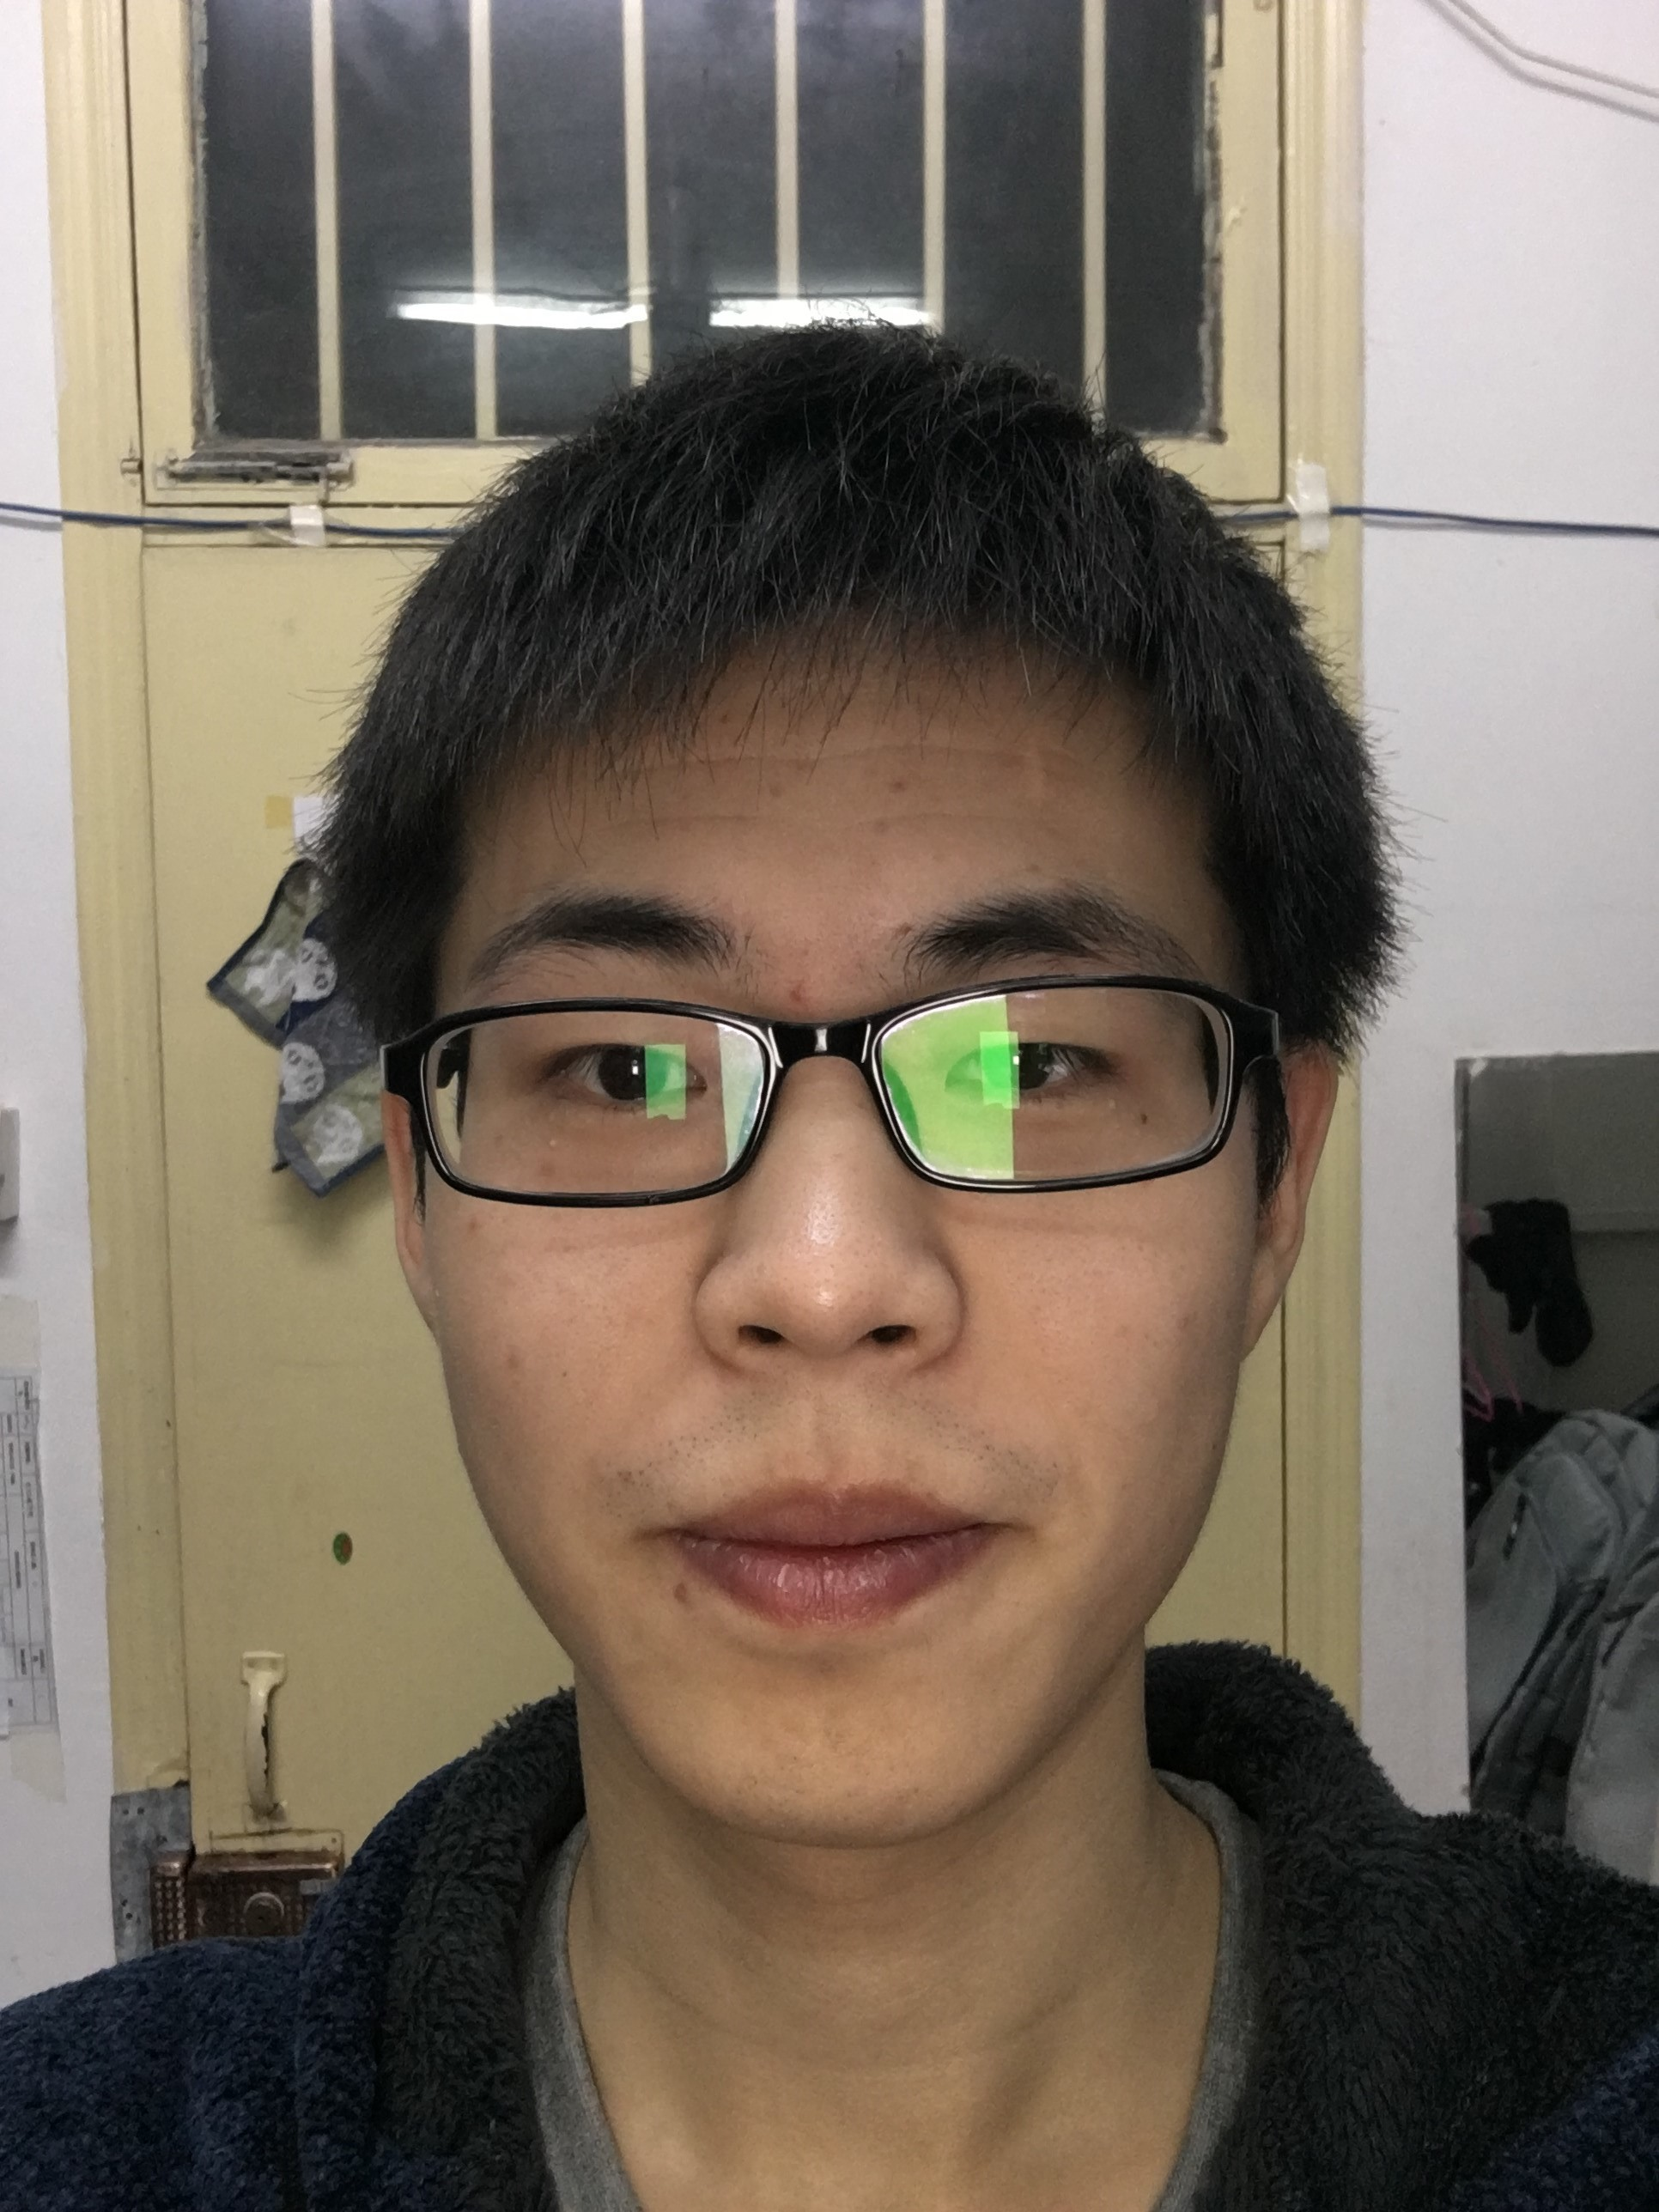
\includegraphics[width=18mm, height=24mm]{../../Figures/lishaogang.jpg} & 
\includegraphics[width=18mm, height=24mm]{../../Figures/Wangyuan.jpg} & 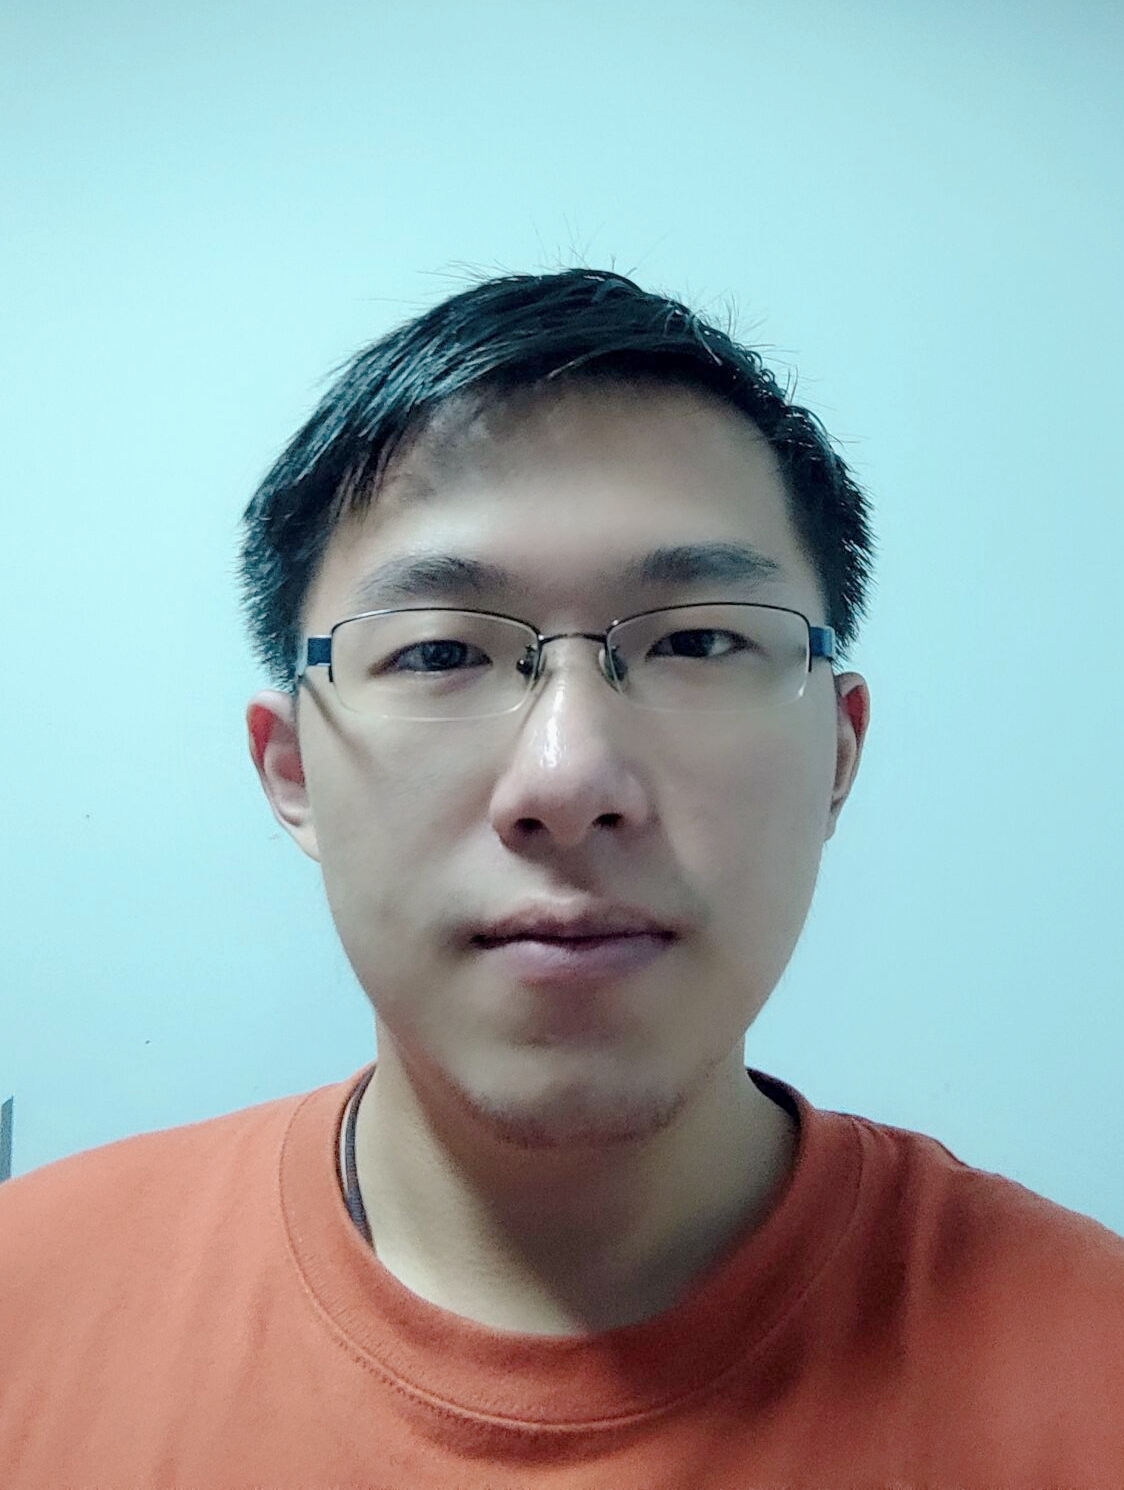
\includegraphics[width=18mm, height=24mm]{../../Figures/Ruanhengyu.jpg} & 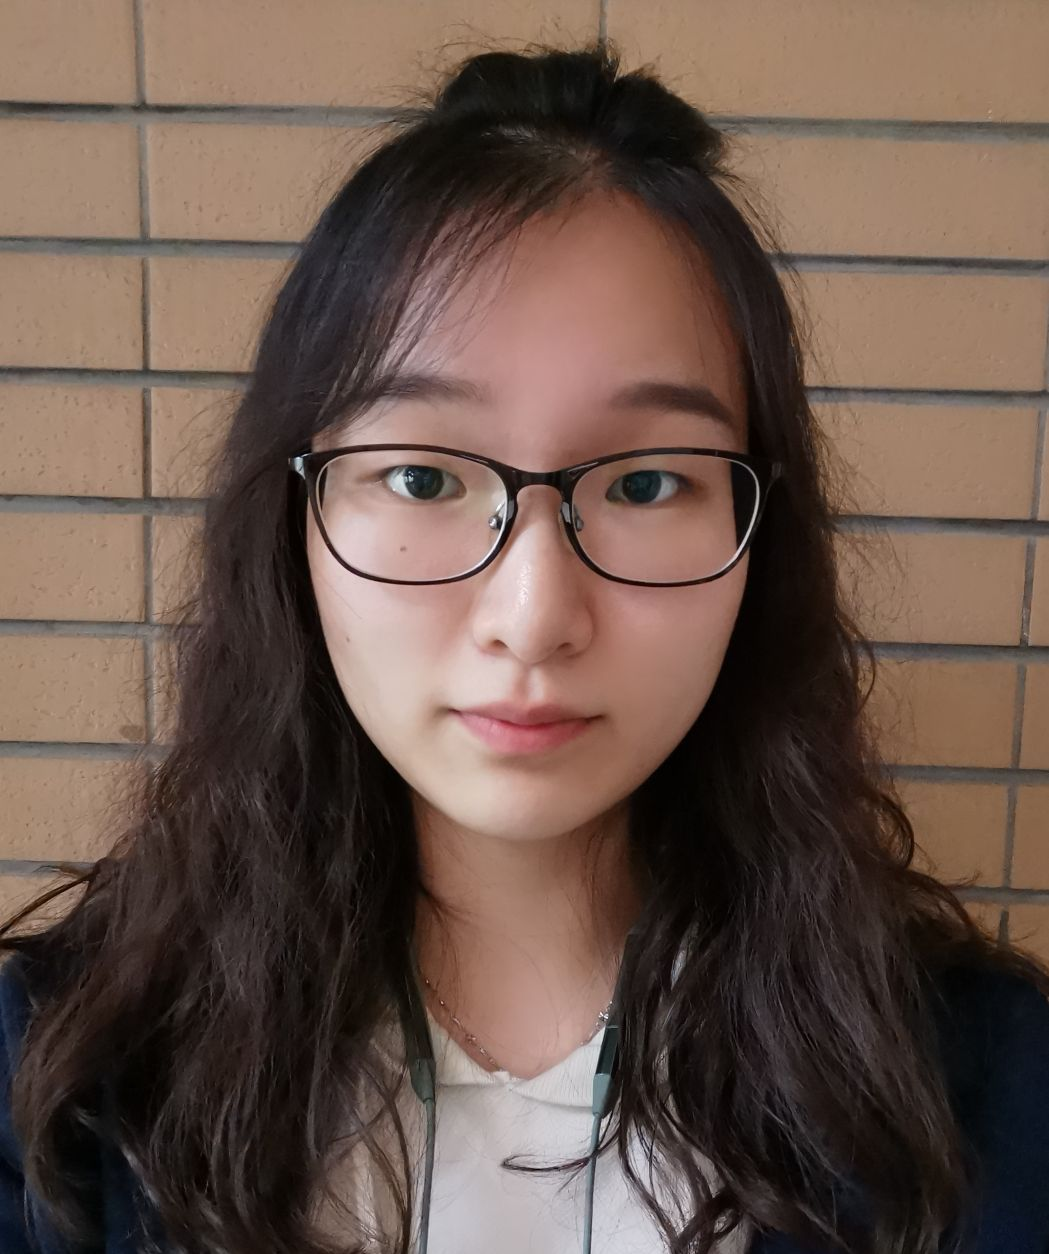
\includegraphics[width=18mm, height=24mm]{../../Figures/Aimee.jpg}\\\hline
		
		\color{blue}\textbf \textrm{Role} & Repository Manager & Data Manager & Bibliography Manager & Document Manager\\\hline
		
		\color{blue}\textbf \textrm{Mession} & \multicolumn{4}{c|}{Define roles , Improve question , Doodle question and Report}\\ \hline
	
	\end{tabular}  

\end{document}
